% 
% Annual Cognitive Science Conference
% Sample LaTeX Paper -- Proceedings Format
% 

% Original : Ashwin Ram (ashwin@cc.gatech.edu)       04/01/1994
% Modified : Johanna Moore (jmoore@cs.pitt.edu)      03/17/1995
% Modified : David Noelle (noelle@ucsd.edu)          03/15/1996
% Modified : Pat Langley (langley@cs.stanford.edu)   01/26/1997
% Latex2e corrections by Ramin Charles Nakisa        01/28/1997 
% Modified : Tina Eliassi-Rad (eliassi@cs.wisc.edu)  01/31/1998
% Modified : Trisha Yannuzzi (trisha@ircs.upenn.edu) 12/28/1999 (in process)
% Modified : Mary Ellen Foster (M.E.Foster@ed.ac.uk) 12/11/2000
% Modified : Ken Forbus                              01/23/2004
% Modified : Eli M. Silk (esilk@pitt.edu)            05/24/2005
% Modified : Niels Taatgen (taatgen@cmu.edu)         10/24/2006
% Modified : David Noelle (dnoelle@ucmerced.edu)     11/19/2014
% Modified : Roger Levy (rplevy@mit.edu)     12/31/2018



%% Change "letterpaper" in the following line to "a4paper" if you must.

\documentclass[10pt,letterpaper]{article}

\usepackage{cogsci}

\usepackage{csquotes}

\cogscifinalcopy % Uncomment this line for the final submission 


\usepackage{hyperref}
\usepackage{xcolor}	
\definecolor{darkblue}{rgb}{0, 0, 0.5}
\hypersetup{colorlinks=true, citecolor=darkblue, linkcolor=darkblue, urlcolor=darkblue}
\renewcommand{\appendixautorefname}{Appendix}

%\usepackage{wrapfigure}
\usepackage{graphicx}

\usepackage{amsmath}

\usepackage{pslatex}
\usepackage{apacite}
\usepackage{float} % Roger Levy added this and changed figure/table
                   % placement to [H] for conformity to Word template,
                   % though floating tables and figures to top is
                   % still generally recommended!

%\usepackage[none]{hyphenat} % Sometimes it can be useful to turn off
%hyphenation for purposes such as spell checking of the resulting
%PDF.  Uncomment this block to turn off hyphenation.


%\setlength\titlebox{4.5cm}
% You can expand the titlebox if you need extra space
% to show all the authors. Please do not make the titlebox
% smaller than 4.5cm (the original size).
%%If you do, we reserve the right to require you to change it back in
%%the camera-ready version, which could interfere with the timely
%%appearance of your paper in the Proceedings.



%\title{Probing Intuitive Physics with Natural Language}
\title{%
  Probing Intuitive Physics Understanding with Natural Language \\
  \large Modeling Human Intuition Using Flexible Queries to Simulated Worlds }
 
\author{{\large \bf Julius Heitkoetter (JULIUSH@Mit.Edu)} \\
  Massachusetts Institute of Technology, 77 Massachusetts Avenue \\
  Cambridge, MA 02139 USA}


\begin{document}

\maketitle


\begin{abstract}
Human intuitions concerning physics are remarkable in their performance and ability to be expressed in natural language. In a heartbeat, humans are able to predict \textit{which direction a tree may fall} even if they have seen very few examples of trees falling. Furthermore, humans are able to express and share these intuitions easily through natural language queries: \textit{How will the tree fall?}, \textit{What will the tree look like after it has fallen?} The ability of humans to reason and communicate physical intuition with relatively few examples outperforms all comparable AI based multimodal and physics engine models. Furthermore, it contributes to one of the biggest open questions in cognitive science: \textit{How do we learn so much with so little?} Modern day research in cognitive science points to hierarchical Bayesian inference as an avenue to solve this problem. In this study, we propose a framework for modeling human intuition using natural language queries which are transformed into a probabilistic language of thought and are used to flexibly probe bayseian inference over a set of simulated worlds. We then show that this framework is able to outperform state-of-the-art multi-modal baselines and exhibit strong correlations to human behavior. 

\textbf{Keywords:} 
Intuitive Physics; Simulated Worlds; Probabilistic Language of Thought; Bayesian World Modeling, Natural Language Processing.

\textbf{Code:} \url{https://github.com/julius-heitkoetter/NaLaPIP}
\end{abstract}


\section{Introduction}

Our intuitive physics understanding is fast and can be efficiently probed using natural language. At a glance, we can tell whether \textit{two cars will collide, a stack of boxes will fall}, or \textit{a child is likely to fall off a playground}. Not only can we make these predictions, we can infer qualitative properties of the world by observing these situations: \textit{how fast are the cars moving, how heavy are the boxes,} or \textit{how strong is the child.} Moreover, these predictions and inferences are able to be communicated and probed extremely efficiently through natural language and with few examples beforehand.

How are we able to perform this inference in so little time, with so few examples? Modern AI models such as state-of-the-art Large Language Models (LLMs) still fall short when it comes to replicating human-like behavior in out-of-distribution tasks \cite{Collins2022StructuredFA}. However, work from \citeA{tenenbaum1999bayesian} outlines a Bayesian framework to answer the question of \textit{how do we learn so much from so little?} More modern work articulates this Bayesian framework as a probabilistic language of thought used to convert word models to world models \cite{2306.12672}.  \citeA{battaglia2013simulation} apply an extension of this Bayesian framework to intuitive physics, showing evidence that human intuitive physics is modeled as probabilistic inference over a mental physics engine. Further work shows evidence of grounding intuitive physics understanding in natural language through the use of probabilistic programs and simulated worlds \cite{zhang2023grounded}. 

In this study, we expand upon the work of these findings to see if we can probe intuitive physics understandings with natural language through a probabilistic language of thought. We seek to build a model using Bayesian frameworks which we can probe with natural language questions in order to extract evidence of human-like intuitive physics in simplified cases. This study seeks to make two main contributions in this direction:
\begin{enumerate}
    \item We propose a framework for converting questions in natural language to a probabilistic programming language (PPL) which is then used to probe intuitive physics models that use simulated worlds and probabilistic language of thought. A high level overview of this framework is illustrated in figure \ref{fig:workflow}
    \item We develop NaLaPIP, a model for \textit{Natural Language Probing of Intuitive Physics} which uses the above framework to answer questions containing a natural language and a visual stimulus. 
\end{enumerate}

\begin{figure}[ht]
  \begin{center}
    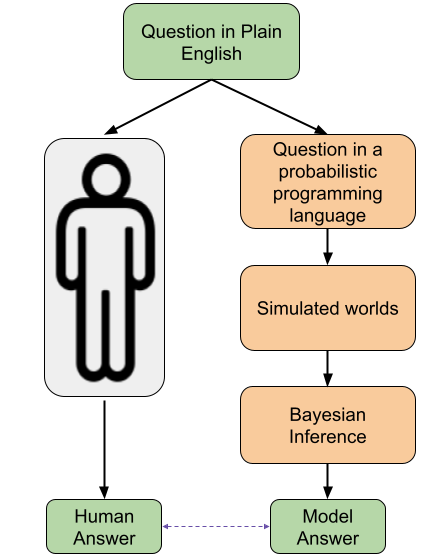
\includegraphics[scale=.36]{images/966_diagram2.png}
  \end{center}
  \caption{An overview of the framework presented in this study. The framework can be modeled as a pipeline, where an intuitive physics question in plain English is converted to a question in a probabilistic programming language, applied to extract answers from simulated worlds, and put through Bayesian inference over all possible worlds to get a distribution of model answers which are compared to human answers. }
  \label{fig:workflow}
\end{figure}

Both of these contributions are inspired by stimuli from \citeA{battaglia2013simulation} and approach from \cite{zhang2023grounded}.

\section{Related Work}

Preview work has focused on constructing linguist meaning from cognitive representations in a compositional language of thought \cite{fodor1975language,jackendoff1985semantics} and further work which addresses the vagueness often found in natural language \cite{van2012probabilistic,cooper2015probabilistic,goodman2015probabilistic}. In our study, we related these findings and developments to intuitive physics problems.

Other work in intuitive physics has explored the ability to use probabilistic inference approaches \cite{smith2013sources,smith2024intuitive} to model human behavior as well as using simulation as an engine of physics scene understanding \cite{battaglia2013simulation}. However, the questions asked in these experiments were often simple, with a the focus of the study on deriving the mechanisms of understanding. In this study, we examine more than just simple questions in simple scenes, but elevate the level of the questions such that they are difficult for humans to answer\footnote{Average human response time in the study we conduct is between 20 seconds and a minute}. 

Lastly, modern approaches to the problem have been able to expand out from simple 2D scenes to complex 3D scenes \cite{xue20233d}. Other work done by \citeA{battaglia2013simulation} pioneers the use of a single model for intuitive physics understanding across 5 different tasks and the work done by \citeA{zhang2023grounded} creates a model which is able to process physical scene descriptions in natural language as input and output distributions of answers over a fixed question. In our study, we build off of similar ideas, but give a fixed scene representation and vary the underlying question. 

\section{Methods}

\begin{figure*}[ht]
    \centering
    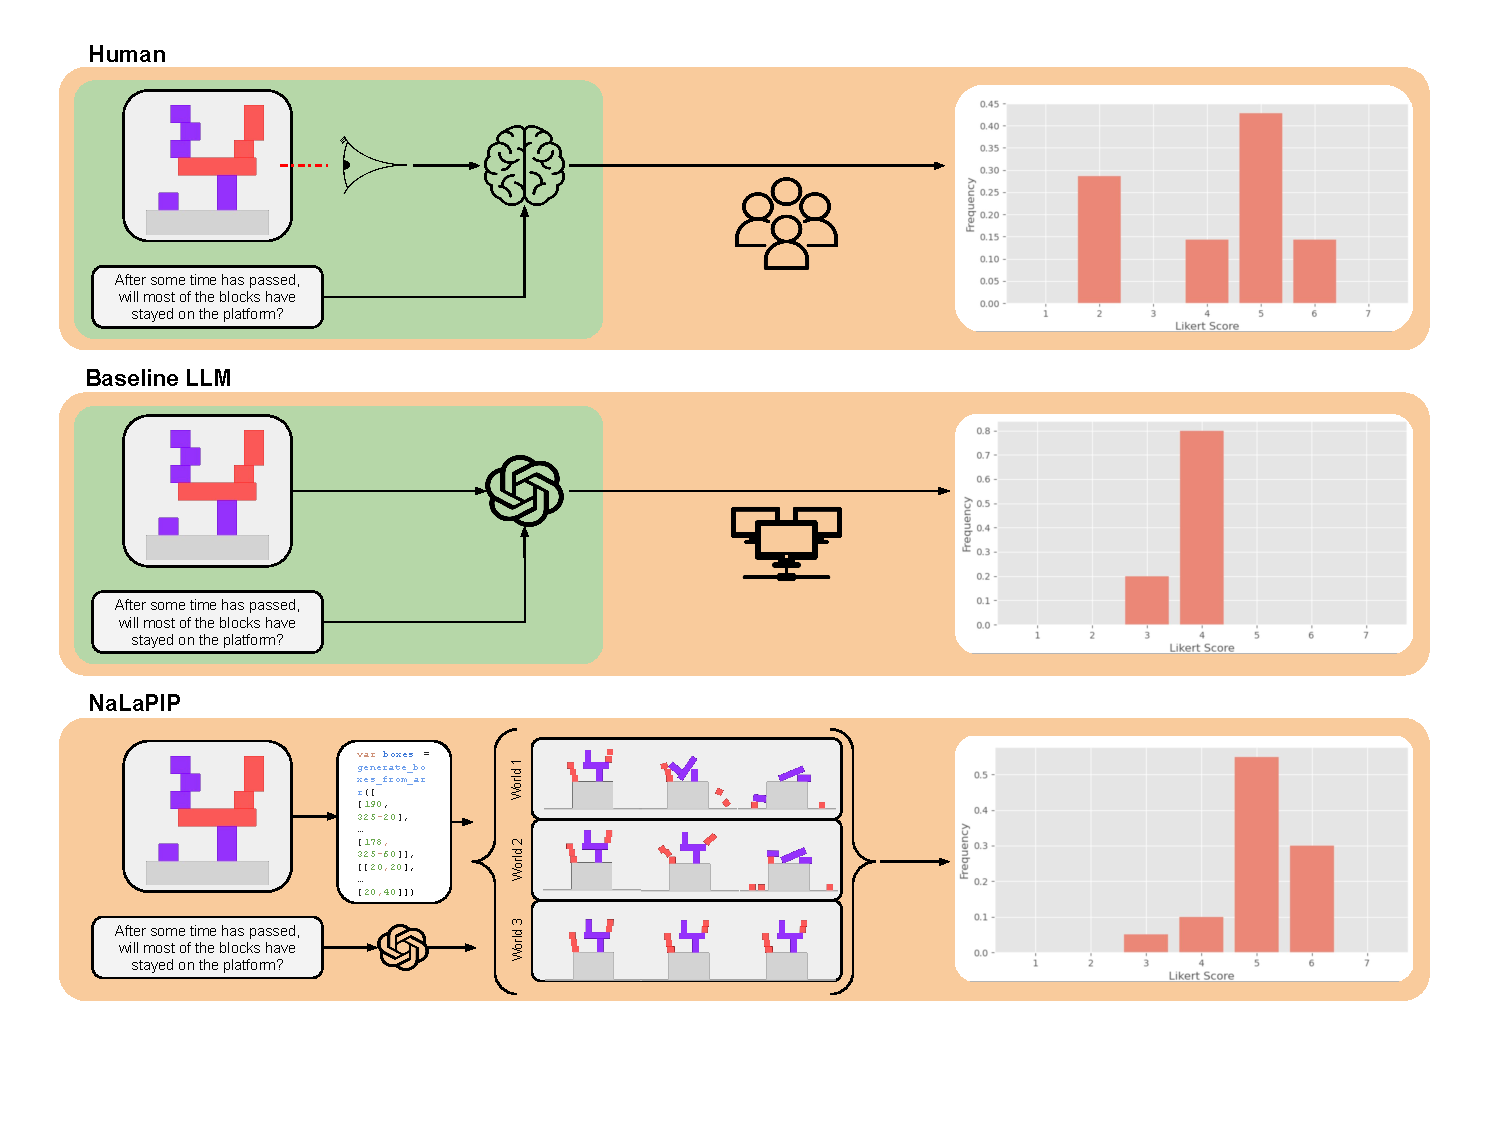
\includegraphics[scale=0.75]{images/966_diagram1.pdf}
    \caption{An outline of how the 3 agents involved in this study respond to stimuli. (Top) A human's visual perception system inputs a visual stimulus which is paired with a natural language stimulus to extract an answer. The answer is aggregated over multiple people to gain a distribution over results. (Middle) A multi-modal large language model is fed an image and natural language text and asked to make an inference of the result. Many calls are used to reconstruct the distribution of logit answers. (Bottom) NaLaPIP converts the inputs to probabilistic language of thought with help by a translating agent and a deterministic visual system. It then performs inference over all possible worlds to generate a distribution over results.}
    \label{fig:NaLaPIP}
\end{figure*}

We begin by presenting an overview of the experiment. Then we describe the stimuli used in the experiment and the process for human data acquisition. Following sections will then discuss our proposed model, NaLaPIP, as well as a baseline model derived directly for Large Language Model outputs. Lastly, we describe post processing applied to both NaLaPIP and baseline LLM data to prepare it for a better fit to human data.

\subsection{Study Overview}

We propose a natural language and intuitive physics task inspired by stimuli from \citeA{battaglia2013simulation} and structure from \citeA{zhang2023grounded}, in which subjects were presented with visual scenes of various stable or unstable stacks of blocks and asked to predict the outcome of the scene after some time had passed. Our study expands on this work by allowing questions to vary flexibly in natural language, converting each question into a piece of probabilistic code and then running that code. Additionally, for simplicity, our scenes are 2-dimensional and we use a simplified approach to physics simulation.

\subsection{Stimuli}

Our stimuli are composed of a question in natural language and a 2D physical scene depicted through an image. 

Each of the 2D physics scenes are composed of a series of blocks, colored red and purple, which are stacked on top of each other on a grey platform. The scenes are designed such that the blocks are stacked in a manner where it is not immediately obvious what will happen after some time has passed and gravity is allowed to act on the stack.\footnote{To check this, we record the average response time from humans when they answer questions about the stack and verify that it is on the order of 10 seconds.} A full set of visual stimuli are included in the appendix \autoref{app:visual_stimuli}. 

Each of the questions are designed to probe intuitive physics understanding of models. The base of the questions always query's what the physical state of the system will be (\textit{will there be more than 3 boxes on the platform}, \textit{will there be an even number of purple boxes on the platform}, etc.) and then is preface with the phrase \textit{After some time has passed} to emphasise the probing of intuitive physics after the simulation has completed.

Questions were built using base units representing conceptual categories widely studied in both cognitive science and natural language processing contexts:
\begin{enumerate}
    \item \textbf{Number:} Asking a question on the number of blocks, such as \textit{three blocks} or asking a question about a very simple arithmetic property of the number of blocks, such as \textit{divisible by 3} \cite{bartsch1973semantics,gelman1978thechild}.
    \item \textbf{Spatial relations:} Asking a question on the block's position relative to other objects in the space, such as \textit{to the left of the platform} \cite{landau1993whence}. 
    \item \textbf{Quantifiers:} Involving statements which imply reasoning about the number of blocks, but do no directly qiery what that number is, such as \textit{some}, \textit{most}, \textit{few}, etc. \cite{montague1973proper,van2021probabilistic, barwise1981generalized}.
    \item \textbf{Gradable adjectives:} Involving adjectives which exist on a scale, such as \textit{tall}, \textit{large}, etc. \cite{klein1980semantics,lassiter2017adjectival}. 
\end{enumerate}
We design 8 of these questions for training and then use a separate 6 for testing. The full set of questions used in this study is included in the appendix \autoref{app:language_stimuli}. 

For the stimuli used in the study, we pair each of the 8 visual stimuli with all 6 of the natural language stimuli, resulting in 48 total stimuli.

\subsection{Human data acquisition} 

In total, 12 responses were gathered from 12 different participants using a online app tracking responses and response time. Participants were asked to rate their responses on a scale from 1 (\textit{Definitely no}) to 7 (\textit{Definitely yes}), known as a \citeA{likert1932technique} scale. To insure the quality of the responses, each participant was first presented with a comprehension check before being presented with 24 different pairs of stimuli. More details on the application are included in the appendix \autoref{app:human_app}.

\subsection{The NaLaPIP model}

In this study, we create and evaluate NaLaPIP: a cognitive model which translates a visual stimuli and a natural language question into probabilistic language of thought (PLoT) \cite{goodman2014concepts} and produces an answer on a \citeA{likert1932technique} scale. The model can be broken up into 3 different components: creating probabilistic generative models from visual stimuli, inserting probabilistic language of thought derived from natural language stimuli, and synthesizing an answer using a physics simulator. The probabilistic generative models are inspired by those proposed by \citeA{battaglia2013simulation}, the probalistic language of thought from natural language is based on the work of \citeA{doi:https://doi.org/10.1002/9781118882139.ch21} on the use of probabilistic techniques in natural language pragmatics, and the fusion of these two techniques into one cohesive model is inspired from work done by \citeA{zhang2023grounded}. 

\subsubsection{Probabilistic generative models from visual stimuli:} We create a probabilistic generative model which generates all possible worlds over a perception prior on the location and size of the blocks. Simple models of vision priors can derived from Gaussian distributions \cite{mamassian2002bayesian,series2013learning}. Therefore, our prior over all possible worlds is based on Gaussian priors on the position and size of each of the blocks. These Gaussian priors are centered at the true value of their corresponding property. Additionally, the position priors are given width $\sigma_{pos}$ and the size prior are given width $\sigma_{size}$. These widths remain as free parameters in the NaLaPIP model. 
The generative model is written in a probabilistic programming language (PPL) named WebPPL, which uses JavaScript based syntax to stochastically generate and sample from all possible worlds \cite{dippl}. 

\subsubsection{PLoT from natural language stimuli:} In order to process the question in the context of our generative model, we need a translation function $f$ where $f: \text{Natural Language} \to \text{PLoT}$. As demonstrated by OpenAI's Codex, LLMs provide a model for approximating this function to a high degree \cite{2107.03374}. For this study, we use GPT-4, a more powerful successor of Codex. Using few-shot prompting \cite{brown2020language}, we give 8 translation examples and some other context and find that the LLM was able to correctly generate 48 out of 48 questions used in the final experiment with very little prompt engineering. More information on prompting can be found in the appendix \autoref{app:NaLaPIPLLM_prompts}. 

\subsubsection{Answer synthesis with a physics simulator:} Once the possible worlds have been generated, they are simulated using a WebPPL based physics model, Box2D \cite{box2d}. The default physics parameters are maintained and the only force which acts is gravity. After the simulation, we create the set of all possible worlds \textit{after} gravity has acted, which we can query and sample from using the PLoT code generated in the previous section. Lastly, the results are interpreted on a \citeA{likert1932technique} scale. 

\subsection{LLM Baseline}

To establish a reference for our results, we create a baseline model. For this baseline model, we choose the mutlimodal version of the LLM used in the NaLaPIP model, GPT 4V. We prompt using a zero-shot prompt and with in-context examples to generate a few-shot prompt \cite{brown2020language}. The few-shot prompt is created with only one image, where the in-context examples are composed of 8 questions from the training set and corresponding answers retrieved from the mean of the human data distribution. More information on the prompts for the baseline can be found in the appendix \autoref{app:BaselineLLM_prompts}. Once we insert the natural language question and image stimulus properly into the prompt, we feed this through the LLM to get a result. In order to achieve a distribution, we pass through the LLM multiple times with \textit{tempaure=t} and combine all the results. The temperature, $t$, is a free parameter if the LLM model and can be tuned accordingly.

\subsection{Post Processing}

After distributions have been obtained from NaLaPIP and the Baseline LLMs, they are transformed through a logistic function in order to help transform the probability space outputted by the models to a human scale. Additionally, this logistic function accounts for non-linearity in human judgement \cite{KIM2008517}. 
We parameterize the logistic function by $(a,b,c,d)$ such that if we have initial model rating of $r$, our post-process model rating $r'$ is given by \autoref{eq:sigmoid} 1. 
\begin{equation}
    r' = \frac{c}{1 + e^{-(ax-b)}} + d
\end{equation}
\label{eq:sigmoid}
We add free variables $(a,b,c,d)$ to the models which will, along with the other free parameters, be fit to human data. A full summary of free parameters of the study can be seen in Table \ref{table:free-parameters}. 

\begin{table}
\begin{center} 
\begin{tabular}{ll} 
\hline
Free Parameter    &  Description \\
\hline
$\boldsymbol{\sigma_{pos}}$      &   Uncertainty from perception on position \\
$\boldsymbol{\sigma_{size}}$      &   Uncertainty from perception on size \\
$\boldsymbol{a}$           &   Sharpness of logistic function \\
$\boldsymbol{b}$           &   Model data offset of the logistic function \\
$\boldsymbol{c}$           &   Scale of logistic function \\
$\boldsymbol{d}$           &   Human data offset of the logistic function \\
$\boldsymbol{t}$           &   Variability in baseline LLM model answers \\
\hline
\end{tabular} 
\caption{Summary of all free parameters used in the experiment and their interpretation. All parameters are free in NaLaPIP model except $\boldsymbol{t}$ and only $\boldsymbol{t}$, $\boldsymbol{a}$, $\boldsymbol{b}$, $\boldsymbol{c}$, and $\boldsymbol{d}$ are free in the LLM baseline model.} 
\label{table:free-parameters} 
\end{center} 
\end{table}

\begin{figure*}[ht]
\hfill
    \parbox{.47\linewidth}{
        \centering
        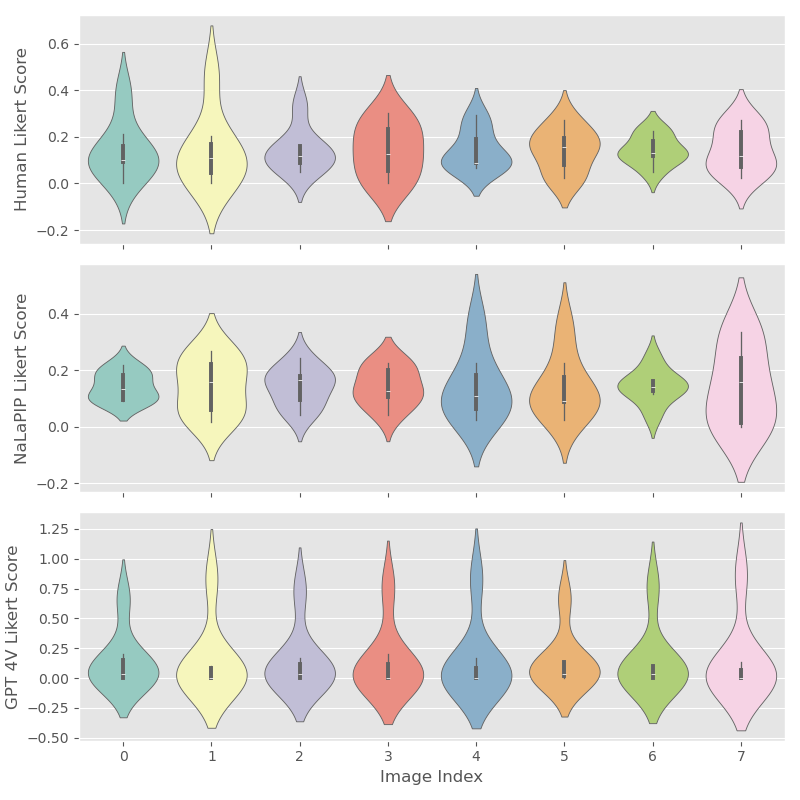
\includegraphics[scale=0.4]{images/stacked_violin_plot.png}
        \label{fig:violin}
    }
    \hfill
    \parbox{.47\linewidth}{
        \centering
        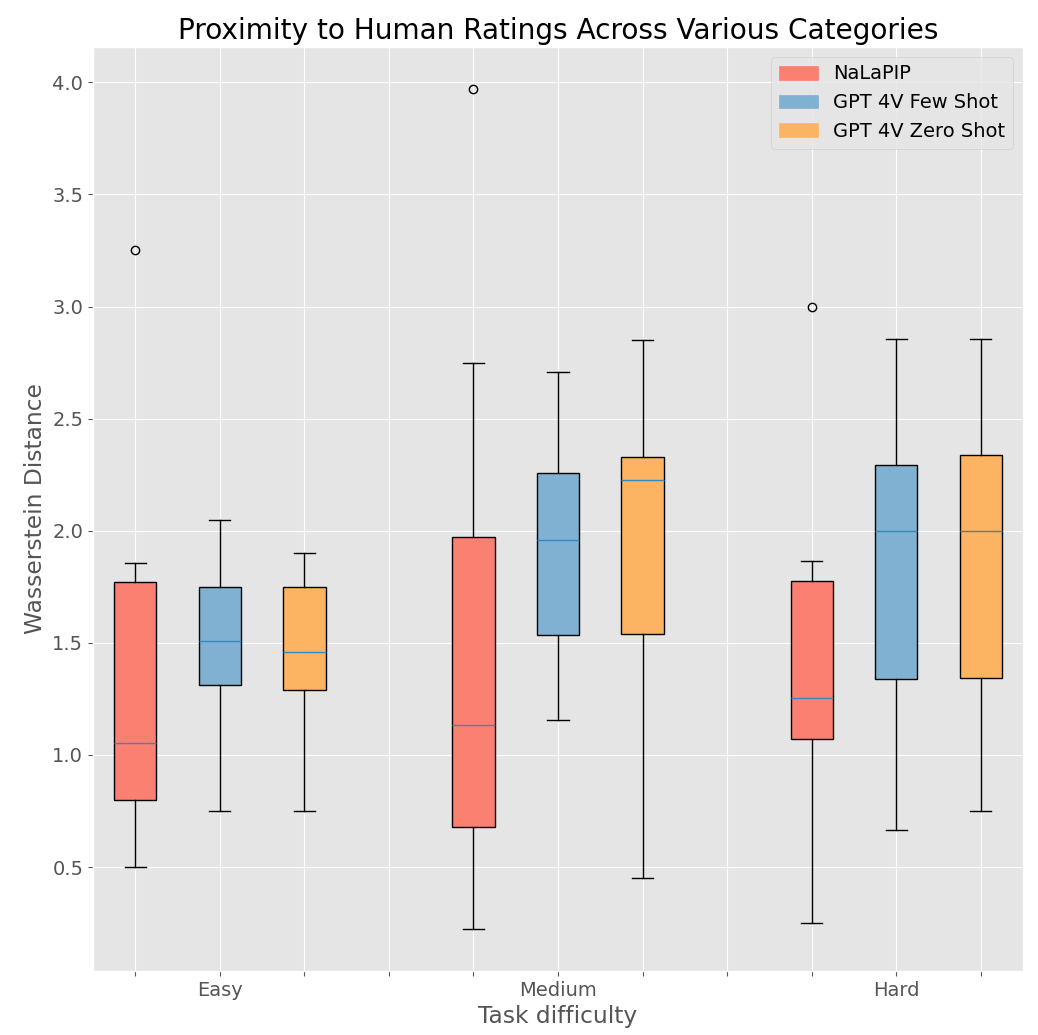
\includegraphics[scale=0.33]{images/wasserstein_distance_by_runtime.png}
        \label{fig:wasserstein_distance_by_runtime}
    }
    \caption{(Left) Violin plot display distribution over human answers (top) NaLaPIP answers (middle) and LLM baseline answers (bottom). Each violin collumn corresponds to a different image stimulus and is averaged over all questions asked about that image stimulus. (Right) Wasserstein distance when compared to human ratings across various difficulties of tasks and various models. Lower Wasserstein distance is interpreted as closer to human ratings.}
\end{figure*}


\section{Results}

In this study, we evaluate the quality of our cognitive model, NaLaPIP, by comparing it to human responses. For reference, we also compare the output of bleeding edge mutlimodal generative model, GPT-4V, to human responses. We evaluate the comparison to human responses by (1) comparing the distance between the average human response and the average model response over all possible stimuli and (2) comparing the distance between the human and model distributions using the Wasserstein metric. In evaluating these metrics, we obtain two main results\footnote{Note, all results shown are with tuned free parameters. The parameters found for NaLaPIP are $\sigma_{\text{pos}} = 3, \sigma_{\text{size}} = 1, a=0.79, b=3.978, c=6.00, d=1.00$. The free parameters found for GPT-4V are surprisingly close at $a=0.78, b=3.975, c=6.00, d=1.00, t=1.5$}:
\begin{enumerate}
    \item NaLaPIP is a \textbf{significant improvement} over state-of-the-art mutlimodal AI models.
    \item Whil there is a \textbf{discrepancy} between exact human and NaLaPIP responses, we can identify a \textbf{strong positive correlation} between the two samples. 
\end{enumerate}

The section on the significant improvement of NaLaPIP focuses on comparing the Wasserstein metric derived from NaLaPIP and GPT-4V responses and outlines the statistical significance of this comparison. The section on the discrepancy between human and NaLaPIP responses focuses on comparing the mean of responses from NaLaPIP and GPT-4V directly as well as their correlation.


\subsection{The improvement of NaLaPIP over GPT 4V:}

We observe significant improve of our model, NaLaPIP, over a baseline state-of-the-art multimodel transformer, GPT-4V. Qualitatively, this is best seen in Figure \ref{fig:violin}, which shows a comparison between distributions of likert scores aggregated over various images\footnote{The mapping between image index and image can be found in the appendix \autoref{app:visual_stimuli}} \footnote{The y-axis labels are not shown on the violin plot is not shown because the distributions are shown after logistic re-scaling, which transforms the axis. Due to the monotonicity of the transformation, higher likert scores are still shown as higher on the axis.}. From this plot, one can qualitatively see that GPT-4V is not able to capture differences between images, while NaLaPIP does a much better job matching the general shape of the human distribution. This provides evidence that compared to the baseline, NaLaPIP is able to much better account for physical scene understanding.

To assess this qualitative trend qualitatively, we introduce the Wasserstein metric, which serves as a distance metric between two distributions. The key property of this metric is that distributions which are more similar to one another have lower Wasserstein metrics and the Wasserstein metric is 0 if and only if the two distributions are the same. We compute 3 Wasserstein metrics for each of the 48 tasks\footnote{A task is a question/image pair. 48 tasks are created from 8 images and 6 questions.} to create a quantitative measurement of the difference between human/NaLaPIP, human/few-shot GPT-4V, and human/zero-shot GPT-4V response distributions. We show the distribution of the Wasserstein metric for each task, grouped by task difficulty, in Figure \ref{fig:wasserstein_distance_by_runtime}. We see that across all levels of task difficulty, NaLaPIP shows significant improvement over GPT 4V Few Shot and GPT 4V Zero Shot across all task difficulties. 

To quantify this observation, we perform a T-test of significance on the Wasserstein scores of NaLaPIP compared to baselines. Due to a low number of tasks, this statistical test is done on all the tasks simultaneously. While the distribution over Wasserstein metrics is not normal, the difference between the Wasserstein scores of NaLaPIP and GPT-4V Few Shot is approximately normal\footnote{See appendix \autoref{app:additional_plots} for distributions over Wasserstein metrics}. Therefore, we can perform a 1-tailed T-test of differences with null hypothosis \textit{there is no difference between Wasserstein metrics of GPT-4V Few Shot and NaLaPIP}. The result of this test gives a value of $p=0.1\%$, showing strong evidence that NaLaPIP is a significant improvement over the state-of-the-art mutlimodel AI baseline in modeling human responses to our stimuli. 

\subsection{Correlation between NaLaPIP and human responses.}

While we are able to use the Wasserstein metric to make claims on the significant improvement of NaLaPIP compared to GPT-4V Few Shot, the irregularity of the distribution obtained on the Wasserstein metric when comparing human to NaLaPIP responses makes it difficult to make conclusions using the metric. Therefore, we propose an analysis on the means of the likert scores obtained from humans and from the NaLaPIP model, asserting that a proximity of means suffices to demonstrate accurate modeling of human responses. 

\begin{figure}[ht]
  \begin{center}
    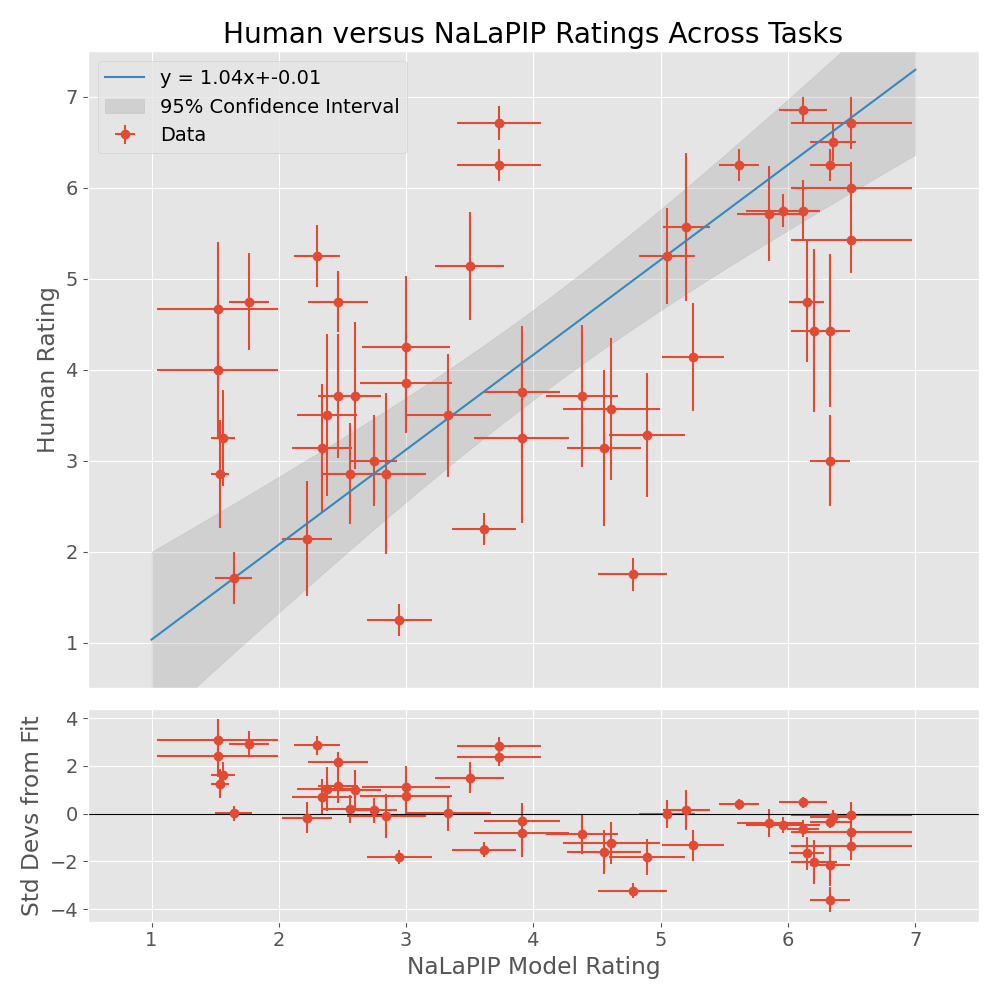
\includegraphics[scale=.32]{images/NaLaPIP_human_scatter_plot_with_deviations.png}
  \end{center}
  \caption{Direct comparison of mean NaLaPIP ratings versus mean human rating (top) and their residuals to line of best fit (bottom). Line of best fit is depicted with a $95\%$ confidence interval assuming data is linear. Confidence interval and residual signify a non-linear relationship.}
  \label{fig:NaLaPIP_scatter_plot}
\end{figure}

Figure \ref{fig:NaLaPIP_scatter_plot} demonstrates the relationship between the mean of the likert distribution of human and NaLaPIP responses over all 48 tasks. We begin analysis of this relationship by assuming a positive linear relationship between mean NaLaPIP likert ratings and mean human likert ratings, performing a linear fit, and propagating the errors of the fit along with the errors on each datapoint to establish a $95\%$ confidence interval. While the best fit demonstrates near equivalence ($y=1.04x -0.01$), we see that far fewer than $95\%$ of the data lies inside this confidence interval. Therefore, we assert that the assumption of a direct linear relationship does not hold for our data. This conclusion is qualitatively echoed by the relationship between residuals and mean NaLaPIP model rating, as displayed in Figure \ref{fig:NaLaPIP_scatter_plot}. 

Instead, we demonstrate that there is a distinct positive correlation between mean NaLaPIP likert scores and mean human likert scores by calculating the $R^2$ metric and it's resultant $p$-value. We find the $R^2$ statistic to be $0.58$ which, when combined with the uncertainty on each data point, results in significance of $p=0.1\%$ that there is no correlation. This leads us to conclude with high confidence that there is a positive correlation between NaLaPIP and human responses\footnote{For comparison, the best LLM baseline result gave a result of $R^2 = 0.114$ with $p=43\%$ significance that there is a correlation. Corresponding plots to this analysis can be found in the appendix \autoref{app:additional_plots}}.




\section{Discussion}

With high statistical significance, we are able to assert that there is a significant improvement of NaLaPIP over state-of-the-art multi-modal LLM baselines and that this is a positive relationship between mean human response and mean likert responses. 
With the improvement over multi-modal LLM baselines, we propose that people's physical scene understanding is explained significantly better by Bayesian inference over simulations on all possible worlds using a perception prior than it is by more general purpose machine learning techniques used to build today's transformers. Furthermore, we show that the framework demonstrated in this study suffices to create a model which correlates strongly with human data over a range of questions and scenes. While this study has a relatively small stimuli sample size, we use the robustness of hyper-parameter adjustments as evidence that the techniques can be applied to a much larger and more diverse set of of stimuli than demonstrated in this study. Lastly, our strong correlations show evidence that intuitive physics models can reflect human behavior by translating natural language questions into probabilistic language of thought sentences which probe Bayesian generative models. 

Our analysis has several limitations. Firstly, we present relatively noisy data over only 48 different tasks. The noise is due a relatively low amount of human participation causing propagation of a large amount on statistical uncertainty throughout the analysis. This lack of human participation also causes the constraint to only 48 tasks, as any more tasks would contribute to a smaller sample size per task. 

Another limitation of our model is the limitation of the prior created over all possible worlds and the simplicity of the Box2D engine used. Work in computational cognitive science has demonstrated several more complex methods for establishing perception and physics priors over intuitive physics models which out-perform the method used in this study \cite{smith2024intuitive}. Furthermore, these models exist in 3D, which would allow the study to be more linked to real-world intuitive physics tasks \cite{xue20233d}. Additionally, this study could be expanded by removing the mapping from a visual image to code which rendered that image through use of inverse graphics methods to construct scene representations to feed into NaLaPIP \cite{yi2018neural}. 

More broadly, we acknowledge the limitations of this study which result weak conclusions about NaLaPIP's ability to exhibit human-like properties. However, we hope this framework will inspire further investigation into probing intuitive physics with natural language. 

\section{Acknowledgments}

I'd like to thank the teaching team of MIT's 9.66 class in the fall of 2023 for their work and dedication to an amazing course in computation cognitive science. I'd also like to specifically thank Josh Tennebaum for his role in inspiring this study with his lectures, office hours advice, and published work. Lastly, I'd like to thank Cedegao Zhang, who's work inspired this study and who gave advice on the framework of the analysis. 

\section{Author Contribution:}

This research paper is the result of the sole efforts and intellectual contribution of Julius Heitkoetter, the sole author of this work. The entirety of the project, including the conception and design of the study, data collection and analysis, interpretation of data, and the writing of the manuscript, was carried out by Julius Heitkoetter with help and guidance from MIT's 9.66 course staff. There were no additional contributors or collaborators involved in any stage of this research project.pro


\bibliographystyle{apacite}

\setlength{\bibleftmargin}{.125in}
\setlength{\bibindent}{-\bibleftmargin}

%\bibliographystyle{latex/bibstyle}
\bibliography{source}

\onecolumn
\appendix

\section{Application Given to Humans During Study}
\label{app:human_app}

The online survey application built with jsPsych \cite{de2023jspsych}. 
\\

\textbf{The instructions were as follows:}

\begin{displayquote}

    Welcome!     We are conducting an experiment about how people evaluate intuitive physics situations when asked a question in plain english. Your answers will be used to inform computer science and cognitive science research.      
          This experiment should take no more than 10 minutes
          
         In this experiment, you will be presented with a series of images containing =stacks of blocks and some simple questions.    
       The block are stacked on a grey platform in a configuration which may or may not be stable.     
       In each situation, you will be asked to imagine what will occur after a sufficiently large amount of time has passed and gravity has finished acting on the stacks of blocks.  ,
       Your task will be to think about how these blocks will fall and their position after they have finished falling=. Note that sometimes, you may be presented with a stable stack where no blocks will fall.    
       You will enter your answer for each question by clicking a rating on a <strong>7-point multiple choice scale</strong> ranging from 1 (definitely no) to 7 (definitely yes).  ,

       You will see descriptions of <strong>24  different scenarios</strong> in total.     

\end{displayquote}

\textbf{The comprehension check was as follows:}

\begin{displayquote}

Check your knowledge before you begin. If you don't know the answers, don't worry; we will show you the instructions again.

What will you be asked to do in this task?

\begin{enumerate}
    \item Look at images containing blocks and answer questions about what is currently occurring in the image.
    \item Look at images containing blocks and answer questions about what will happen in the image after gravity has acted on the blocks.
    \item Look at images containing blocks and answer questions about what will happen in the image while gravity is acting on the blocks.
\end{enumerate}

How will you be providing your answer?

\begin{enumerate}
    \item By writing text.
    \item By selecting an option from a multiple choice scale.
    \item By moving a slider.
\end{enumerate}
    
\end{displayquote}

\textbf{An example presentation of the stimulus was as follows:}

\begin{center}
    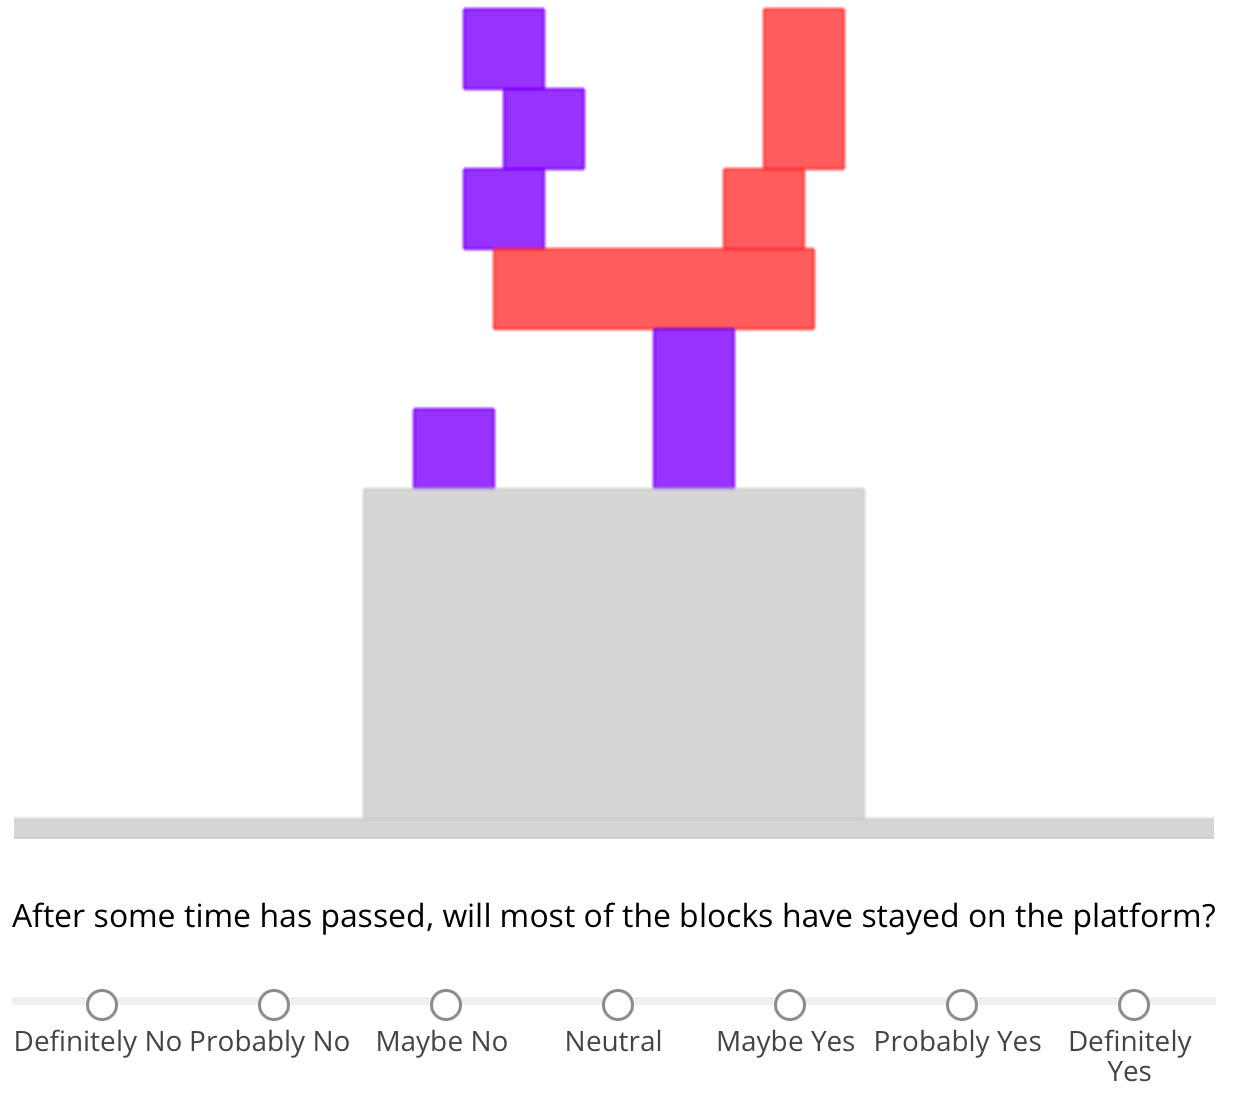
\includegraphics[scale=.2]{images/IMG_1108.jpeg}
\end{center}


\newpage
\section{Prompts used by NaLaPIP to give to LLM}
\label{app:NaLaPIPLLM_prompts}

Below is the prompt that was fed into NaLaPIP's codex to generate sentences in WebPPL (a probalistic programming language) from sentences in natural language

\begin{displayquote}
    You will output code to a probabilistic programming language built in java script. The code you output will be a conditional for a world that starts with 8 purple and blue boxes, stacked on top of each other, on a platform. Please only output a single line of code, nothing else.

Below are the following are the predicates you may use. You can only use these predicates, do not invent other predicates.

var isOnPlatform = function(obj) {{
    return obj.y < 325;
  }}
  
  var isNotOnPlatform = function(obj) {{
    return !(obj.y < 325);
  }}
  
  var isLeftOfPlatform = function(obj) {{
    return obj.y > 325 and  obj.x < 175;
  }}
  
  var isNotLeftOfPlatform = function(obj) {{
    return !(obj.y > 325 and obj.x < 175);
  }}
  
  var isRightOfPlatform = function(obj) {{
    return obj.y > 325 and obj.x > 425;
  }}
  
  var isNotRightOfPlatform = function(obj) {{
    return !(obj.y > 325 and obj.x > 425);
  }}
  
  var isPurple = function(obj) {{
    return obj.color=="purple";
  }}
  
  var isRed = function(obj) {{
    return obj.color=="red";
  }}
  
  var isLarge = function(obj) {{
    return obj.dims[0] > 25 || obj.dims[1] > 25;
  }}
  
  var isNotLarge = function(obj) {{
    return !(obj.dims[0] > 25 || obj.dims[1] > 25);
  }}

  Below are some examples:

  English: After some time has passed, will some of the purple blocks have fallen off the platform. 
  
  Code: filter(isNotOnPlatform, filter(isPurple, finalBoxes)).length > 0
  
  ... [MORE EXAMPLES HERE] ...
  
  English: After some time has passed, will there be more red boxes to the left of the platform than purple boxes on the platform?
  
  Code: 
\end{displayquote}

\newpage
\section{Prompts used by Baseline to give to LLM}
\label{app:BaselineLLM_prompts}

Below are the prompts used to query the GPT-4V baseline LLM \\.
\\
\textbf{Zero Shot Prompt}
\begin{displayquote}
    Look at the 2-D physics scenario in the image. It portrays a set of blocks (purple and red) sitting on a grey platform.

The blocks may be stacked stably or unstably. For a sufficiently long amount of time, gravity is allowed to act on the blocks.

Your job is to answer the following question on a 1-7 scale, with 1 being “Definitely No” and 7 being “Definitely Yes”. 

Only answer "1" or "7" if you are extremely sure about the outcome of the question, as it pertains to the image.

Question as it pertains to image:
\end{displayquote}.
\\
\textbf{Few Shot}
\begin{displayquote}
    Look at the 2-D physics scenario in the image. It portrays a set of blocks (purple and red) sitting on a grey platform.

The blocks may be stacked stably or unstably. For a sufficiently long amount of time, gravity is allowed to act on the blocks.

Your job is to answer the following question on a 1-7 scale, with 1 being “Definitely No” and 7 being “Definitely Yes”. 

Only answer "1" or "7" if you are extremely sure about the outcome of the question, as it pertains to the image.

Question as it pertains to image: "After some time has passed, will there be any red blocks remaining on the platform?"

Rating: 5

... [MORE EXAMPLES HERE] ...

Question as it pertains to image:

Rating:
\end{displayquote}

\newpage
\section{Natural Language Stimuli Used in Study}
\label{app:language_stimuli}

Below are the natural language stimuli used in the study:
.
\\
\textbf{Testing Questions}
\begin{displayquote}
\begin{enumerate}
\item After some time has passed, will there be any red blocks remaining on the platform?
\item After some time has passed, will there be more red blocks to the left of the platform that purple blocks to the right of the platform?
\item After some time has passed, will most of the blocks have stayed on the platform?
\item After some time has passed, will there be any purple blocks to the right of the platform?
\item After some time has passed, will the number of blocks on the platform be divisible by 3?
\item After some time has passed, will the majority of the large boxes be on the platform?
\end{enumerate}
\end{displayquote}.
\\
\textbf{Training Questions}
\begin{displayquote}
    \begin{enumerate}
        \item After some time has passed, will there be more than 3 boxes on the platform?
\item After some time has passed, wil there be any boxes to the left of the platform?
\item After some time has passed, will there be more than 2 red boxes on the platform?
\item After some time has passed, will there be more red boxes to the left of the platform than purple boxes?
\item After some time has passed, will there be any large boxes to the left of the platform?
\item After some time has passed, will most of the boxes have fallen off of the platform?
\item After some time has passed, will there be an even number of purple boxes on the platform?
\item After some time has passed, will some of the purple blocks have fallen off the platform.
    \end{enumerate}
\end{displayquote}

\newpage
\section{Visual Stimuli Used in Study}
\label{app:visual_stimuli}

Below are the visual stimuli used in the experiment. Each caption depicts the corresponding stimulus index which the ensemble of boxes is mapped to.

\begin{figure}[h]
    \parbox{.47\linewidth}{
        \centering
        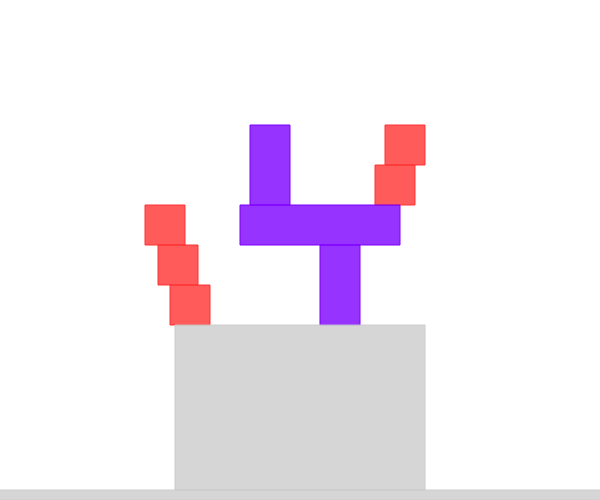
\includegraphics[scale=0.3]{images/ensemble0.png}
        \caption{Visual Stimuli 00}
        \label{table:llama7B-fixed-deceiver-correlation}
    }
    \hfill
    \parbox{.47\linewidth}{
        \centering
        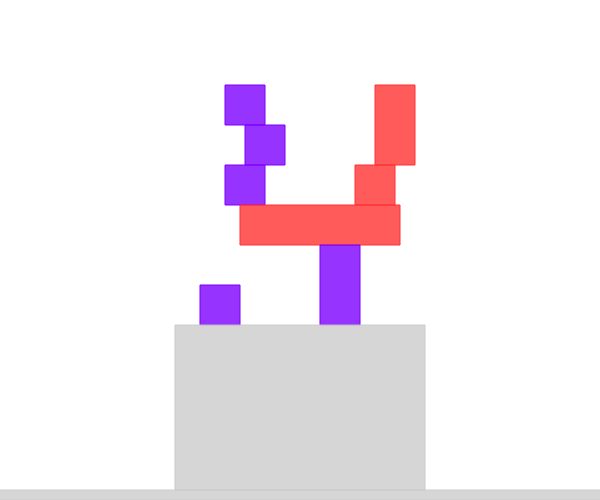
\includegraphics[scale=0.3]{images/ensemble1.png}
        \caption{Visual Stimuli 01}
        \label{table:llama13B-fixed-deceiver-correlation}
    }
\end{figure}

\begin{figure}[h]
    \parbox{.47\linewidth}{
        \centering
        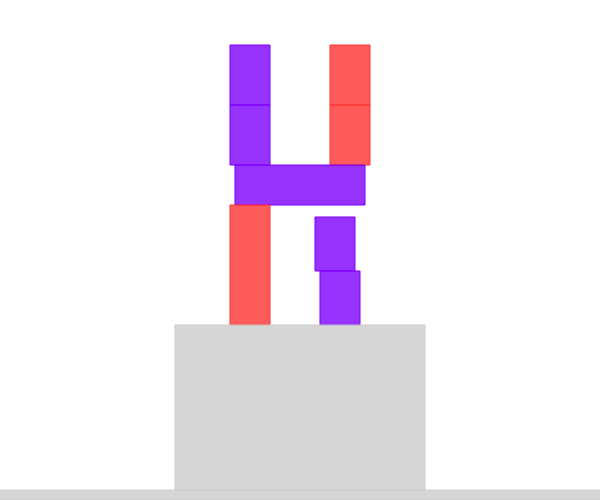
\includegraphics[scale=0.3]{images/ensemble2.png}
        \caption{Visual Stimuli 02}
        \label{table:llama70B-fixed-deceiver-correlation}
    }
    \hfill
    \parbox{.47\linewidth}{
        \centering
        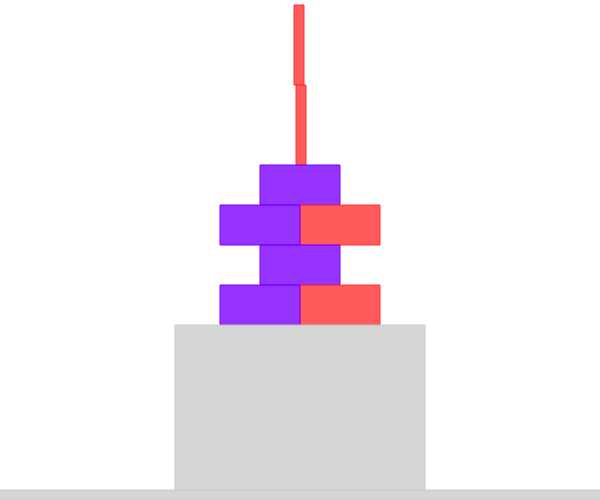
\includegraphics[scale=0.3]{images/ensemble3.png}
        \caption{Visual Stimuli 03}
        \label{table:gpt35-fixed-deceiver-correlation}
    }
\end{figure}

\newpage

\begin{figure}[h]
    \parbox{.47\linewidth}{
        \centering
        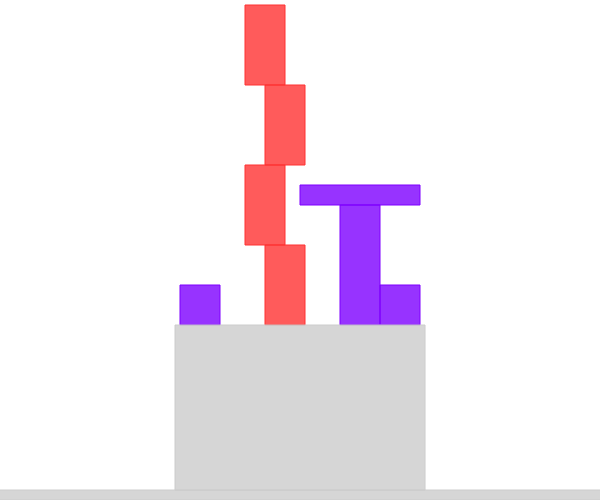
\includegraphics[scale=0.3]{images/ensemble4.png}
        \caption{Visual Stimuli 04}
        \label{table:llama70B-fixed-deceiver-correlation}
    }
    \hfill
    \parbox{.47\linewidth}{
        \centering
        
\includegraphics[scale=0.3]{images/ensemble5.png}
        \caption{Visual Stimuli 05}
        \label{table:gpt35-fixed-deceiver-correlation}
    }
\end{figure}

\begin{figure}[h]
    \parbox{.47\linewidth}{
        \centering
        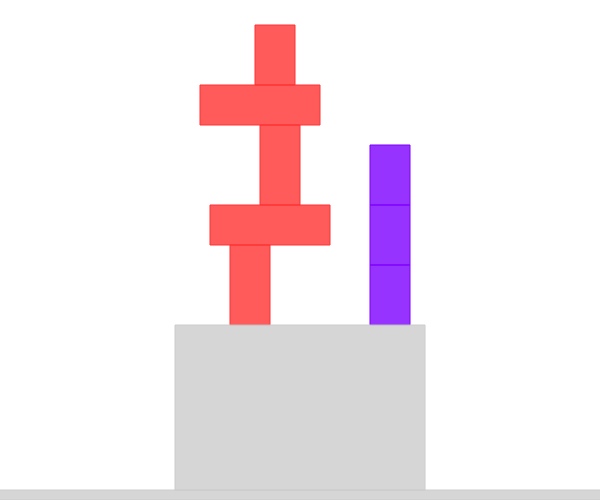
\includegraphics[scale=0.3]{images/ensemble6.png}
        \caption{Visual Stimuli 06}
        \label{table:llama70B-fixed-deceiver-correlation}
    }
    \hfill
    \parbox{.47\linewidth}{
        \centering
        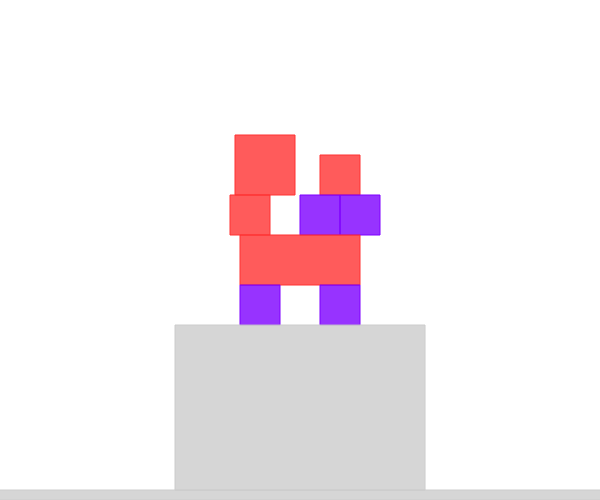
\includegraphics[scale=0.3]{images/ensemble7.png}
        \caption{Visual Stimuli 07}
        \label{table:gpt35-fixed-deceiver-correlation}
    }
\end{figure}

\newpage
\section{Supplemental Plots}
\label{app:additional_plots}

Below are supplemental plots mensioned in the study but not integral to its results.

\begin{figure}[h]
\hfill
    \parbox{.47\linewidth}{
        \centering
        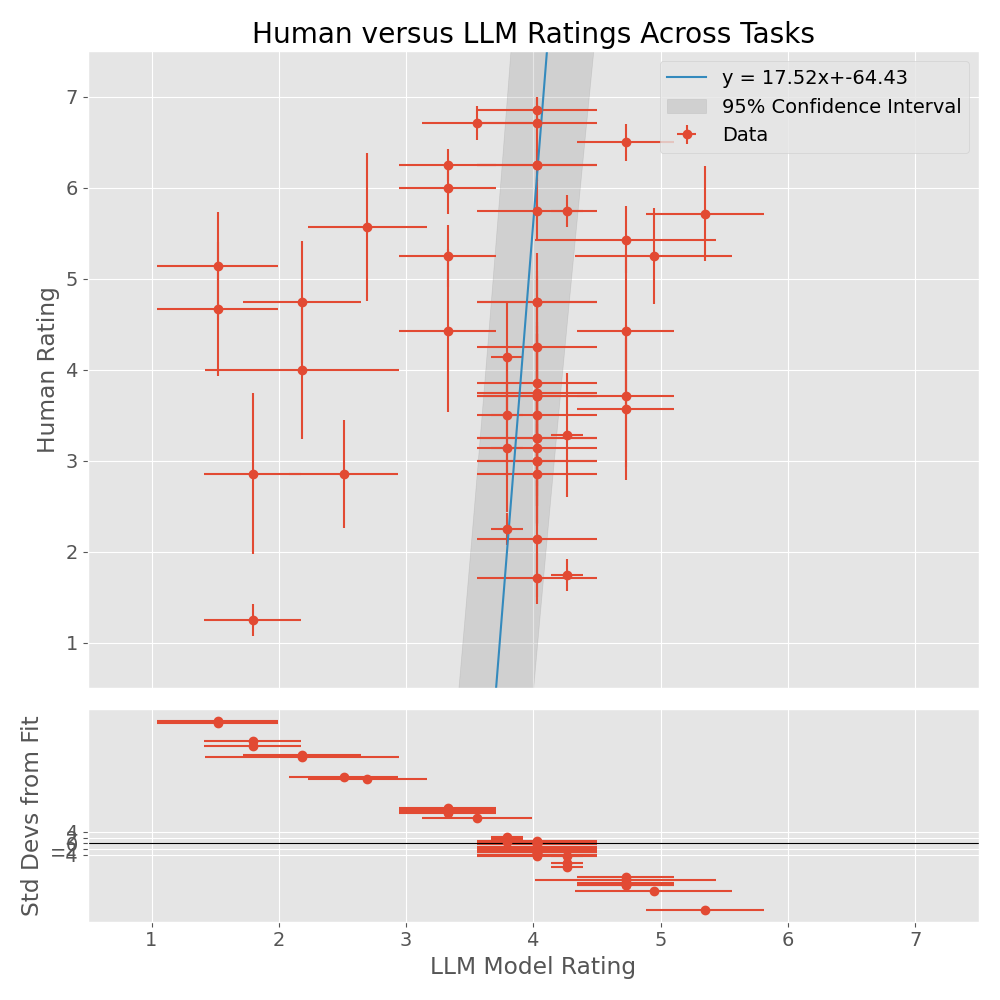
\includegraphics[scale=0.30]{images/LLM_human_scatter_plot_with_deviations.png}
        \label{fig:violin}
        \caption{Direct comparison of mean GPT-4V Few-Shot ratings versus mean human rating (top) and their residuals to line of best fit (bottom). Line of best fit is depicted with a $95\%$ confidence interval assuming data is linear. Confidence interval and residual signify a non-linear and uncorrelated relationship.}
    }
    \hfill
    \parbox{.47\linewidth}{
        \centering
        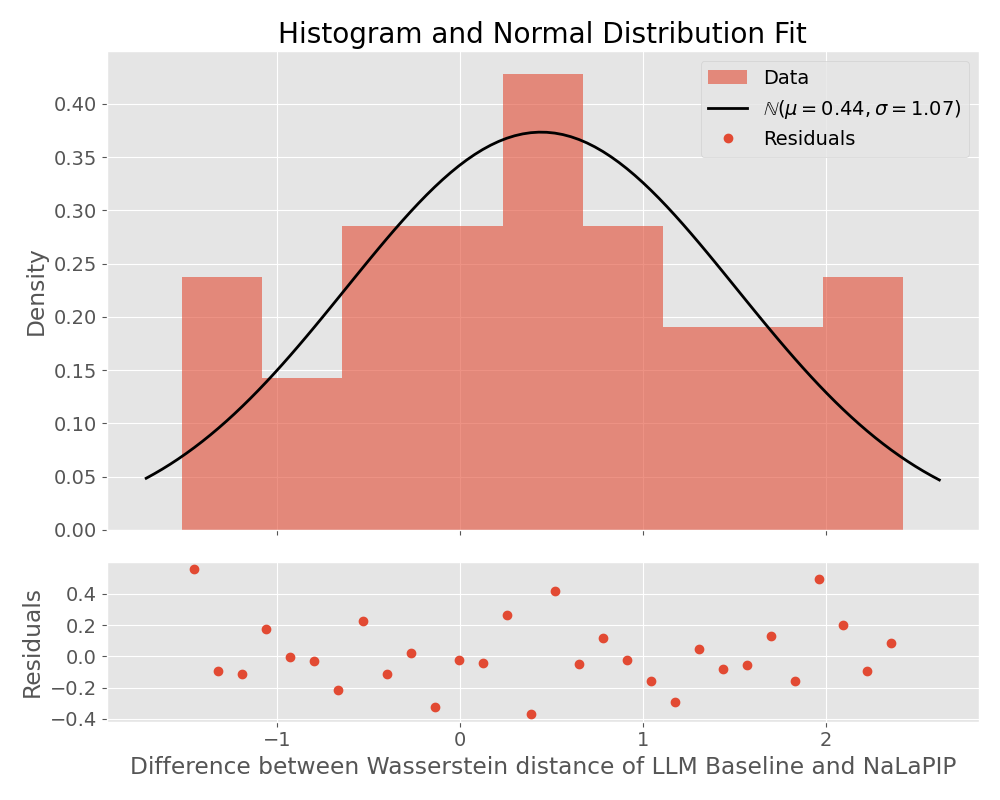
\includegraphics[scale=0.35]{images/wasserstein_difference.png}
        \label{fig:wasserstein_distance_by_runtime}
        \caption{Histogram of task-by-task difference between Wasserstein metric of LLM GPT-4V Few Shot and NaLaPIP when compared with human ratings as well as normal distribution fit. Notice the randomness amoung the residuals signifying an approximately normal distribution. }
    }
\end{figure}

\begin{figure}[h]
\centering
        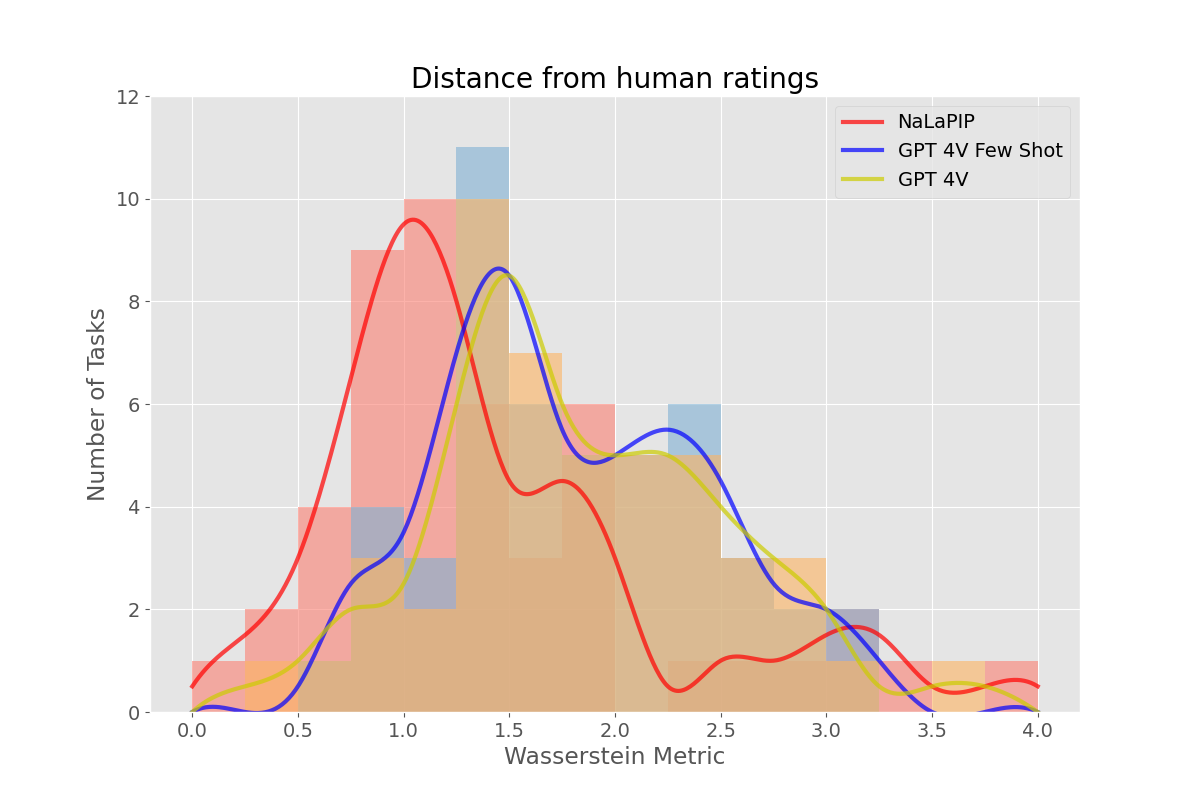
\includegraphics[scale=0.25]{images/wasserstein_distance.png}
        \label{fig:wasserstein_distance_by_runtime}
        \caption{Plot of histograms and spline fits of Wasserstein distance for NaLaPIP (red), GPT-4 Few-Shot (yellow), and GPT Zero-Shot (blue) when they are compared to human data. NaLaPIP shows the best result, with GPT4V Few Shot only slightly outperforming GPT-4V Zero Shot. Note the extremely non-gaussian functional shape.}
\end{figure}




\end{document}
